\section{Техническое задание}
\subsection{Основание для разработки}

Основанием для разработки является задание на выпускную квалификационную работу бакалавра "<Программная система для разработки приключенческих игр">.

\subsection{Цель и назначение разработки}

Основной задачей выпускной квалификационной работы является разработка программной системы приключенческих игр для продвижения их популярности. Данный программный продукт предназначен для демонстрации практических навыков, полученных в течение обучения.

Целью данной разработки является создание программной системы для разработки приключенческих игр и популяризация этого игрового жанра.

Задачами данной разработки являются:
\begin{itemize}
\item проектирование интерфейса;
\item разработка архитектуры приложения;
\item проектирование игрового сценария;
\item реализация взаимодействия приложения с пользователем;
\item реализация графики приложения;
\item реализация сохранений действий персонажа;
\end{itemize}

\subsection{Требования пользователя к движку}

Движок должен включать в себя:
\begin{itemize}
    \item загрузку локаций;
    \item загрузку диалогов;
    \item загрузку объектов в их актуальном состоянии;
    \item сохранение состояний игровых объектов;
    \item возможность изменения сюжета игры;
    \item сохранение действий персонажа;
    \item возможность смены изображений игровых объектов.
\end{itemize}

Композиция шаблона игры, созданной на движке, представлена на рисунке ~\ref{maket:image}.

\begin{figure}[ht]
\includegraphics[width=1\linewidth]{maket}
\caption{Композиция шаблона интерфейса игры}
\label{maket:image}
\end{figure}
%\vspace{-\figureaboveskip} % двойной отступ не нужен (можно использовать, если раздел заканчивается картинкой)

\subsection{Правила игры}

Главный герой игры (ГГ) перемещается по локациям и выполняет квесты. Внутри каждой локации (кроме комнаты ГГ) имеется еще 2-3 подлокации. Начинается игра с предыстории в виде текста в диалоговой панели, который пользователь должен прочесть. Далее персонаж попадает в другие локации, перемещаясь по ним. Для того, чтобы пройти игру, нужно выполнить все квесты. Изначально не все локации доступны для посещения, а только те,что необходимы для текущего квеста. В игре присутствует цепочный механизм заданий, который предполагает последовательность действий (нельзя приступить к следующему заданию, не выполнив предыдущее).
Процесс выполнения квеста заключается в поиске определенных предметов, взаимодействии с персонажами, предметами и локациями игрового мира. Выполнив необходимые действия ГГ дальше двигается по квесту. Игрок может взаимодействовать с игровым миром с помощью компьютерной мыши. При наведении на активный объект курсор мыши поменяет состояние и по нему можно будет понять, с каким объектом мы имеем дело. Доступны следующие объекты взаимодействия с игроком:
\begin{enumerate}
\item Дверь – при наведении курсора иконка указателя меняется на уменьшенное изображение двери. При нажатии на дверь меняется локация.
\item Сущность – при наведении курсор меняется. При нажатии открывается диалог.
\item Предмет – при наведении на него курсор меняется на руку. При нажатии предмет исчезает с карты и появляется в инвентаре.
\item Переход на другую локацию – при наведении иконка курсора меняется на стрелку в направлении доступной локации, в которую хочет перейти пользователь.
\end{enumerate}
Инвентаря как такового нет. С ним нельзя взаимодействовать напрямую. Например, если при нажатии на какой-то объект требуется предмет в наличии у гг и его в инвентаре нет, то выйдет соответствующее сообщение, иначе – гг продвинется по квесту и получит другое сообщение.
По завершению финального квеста игры и прохождению всех локаций пользователь видит развязку сюжета, это конец игры.

\subsection{Сюжет игры}

Главная героиня засыпает и оказывается в одной из локаций игры – в лесу. Там ее пугает обиатель, и она решается выйти из сна, но у нее не получается. Тогда она начинает изучать лес и сталкиваясь с его обитателями, пытается узнать у них, как ей проснуться. Персонажи дают ей квесты, например, принести что-то или чем-то помочь. По выполнении очередного квеста она получает полезную информацию, предмет или пропуск на следующую локацию. В конце концов, она оказывается у хозяина этих земель, который должен ей помочь проснуться.После краткого диалога он убивает героиню, и она просыпается в кровати.

\subsection{Эпизод 1: Лес}

Оказываемся в сумеречном лесу и осмариваемся. Неподалеку видим призрака, подходим к нему и нажимаем для взаимодействия. Девочка подмечает, призрак достаточно милый и не страшный. Начинается диалог с призраком, по окончанию которого призрак моментально увеличивается в размерах и строит страшную гримасу. Девочка пугается и убегает на другую локацию внутри леса - кладбище. Также, она понимает, что у нее не получается выйти из сна. На кладбище видим статую плачущего ангела. Когда подходим к ней, слышим звуки плача. Нажимаем на призрака и в ходе диалога выясняется, что статуя потеряла очень важную вещь в лесу и не может ее найти, тк обездвижена. Взамен на эту вещь статуя обещает помочь выбраться из сна. Не найдя эту вещь в данной части леса, движемся в единственную доступную - начальную, где мы встретили призрака. Увидев призрака, девочка опять испугалась, но не убежала. При осмотре этой локации понимаем, что нужного нам предмета здесь нет, однако достаточно большую часть карты занимает огромный призрак, которого нужно как-то прогнать или уменьшить. Девочка не придумала ничего лучше, как напугать его. Кликаем по ней и смотрим, как она увеличивается в размерах и меняется в лице. Тем временем, по мере увеличения девочки, призрак уменьшается и в конце концов приходит в прежнюю милую форму, а вскоре и совсем убегает. Замечаем, что он закрывал собой тот самый предмет, который мы искали. Забираем его и приносим статуе. Та нас благодарит и говорит, что единственный, кто может помочь ей выбраться из сна - правитель этих земель, а дорогу к нему знает только лис, который спит в этом лесу. Нам открывается путь на следующую локаци этого леса - логово лиса. Зайдя на нее видим большую морду спящего животного. Для того чтобы его разбудить, нужно 3 раза нажать на него. Лис соглашается помочь девочке и провести ее к правителю, но взамен он просит помочь ему с его проблемой: в него что-то залезло и постоянно мешает жить. Лис предлагает девочке залесть к нему в пасть и посмотреть, что там. Нажимаем на пасть лиса и оказываемся в новой локации. Основные объекты и способы  взаимодействия с ними (при нажатии):
\begin{enumerate}
	\item Призрак - говорить.
	\item Статуя - говорить (получить квест), отдать предмет.
	\item Венок – взять, отдать статуе.
	\item Главный герой - вырасти и напугать призрака.
	\item Переход на другую локацию – перейти к призраку, статуе, лису или в пасть к лису.
	\item Лис - разбудить, говорить.
\end{enumerate}

\subsection{Интерфейс пользователя}

На основании анализа предметной области в программе должны быть реализованы следующие прецеденты:
\begin{enumerate}
\item Перемещение по локациям;
\item Перемещение персонажа по игровой области;
\item Просмотр кат-сцен;
\item Просмотр диалогов;
\item Взаимодействие с игровыми объектами при помощи компьютерной мыши.
\end{enumerate}
Таким образом, на рисунке ~\ref{prec:image}сформированы следующие действия пользователя и их последствия.
\begin{figure}[ht]
	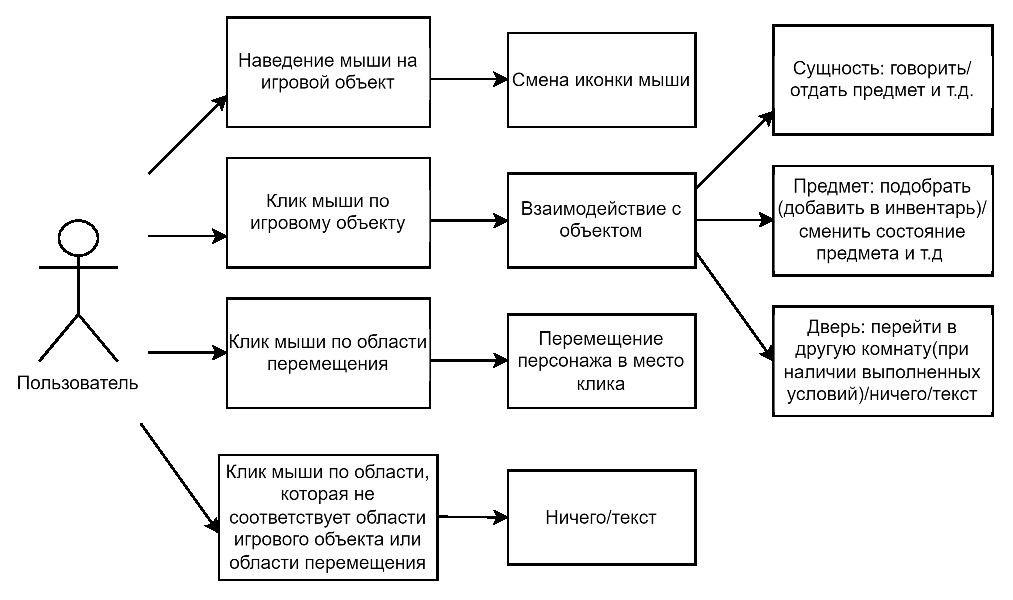
\includegraphics[width=1\linewidth]{prec}
	\caption{Шаблон интерфейса игры}
	\label{prec:image}
\end{figure}
%\vspace{-\figureaboveskip} % двойной отступ не нужен (можно использовать, если раздел заканчивается картинкой)

\subsection{Требования к оформлению документации}

Разработка программной документации и программного изделия должна производиться согласно ГОСТ 19.102-77 и ГОСТ 34.601-90. Единая система программной документации.
